\documentclass[10pt,letterpaper]{article}
\usepackage[utf8]{inputenc}
\usepackage{amsmath}
\usepackage{amsfonts}
\usepackage{amssymb}
\usepackage{graphicx}

\usepackage{algorithm}
\usepackage{algorithmicx}
\usepackage{algpseudocode}


\newcommand{\R}{\mathbb{R}}
\renewcommand{\thesubsection}{\thesection.\alph{subsection}}

\author{Brock Ellefson, Seth Severa}
\title{CSCI432 GW3}
\begin{document}
\maketitle
\section{ Solve the following recurrences:}
\subsection{Show that T(n) = T(n?1)+n is O(n$^{2}$) using the substitution method}
Prove that $T(n) = T(n-1) + n$ is in $O(n^2)$ complexity.\\
We begin by guessing that $T(n)$ is in $O(n^2)$\\
For the base case of n = 1, it's trivial to see that there exists a c where $1 < c1^2$ \\
For $ n > 1$, we have \\
$T(n) = T(n-1) + 1 \leq c(n-1)^2 + n = cn^2 - n(2c-1) + c$ \\
We can see that this last simplification is less than $cn^2$ for some positive n and c. Since we are limiting our $n > 1$ already, we meet the requirement that there does exist some c where $T(n) < c n^2$. \\
Thus, by induction, $T(n) is O(n^2).$

\subsection{Use a recursion tree to determine a good asymptotic upper bound for T(n) = T(n/2) + n$^{2}$}
	\begin{figure}[h]
		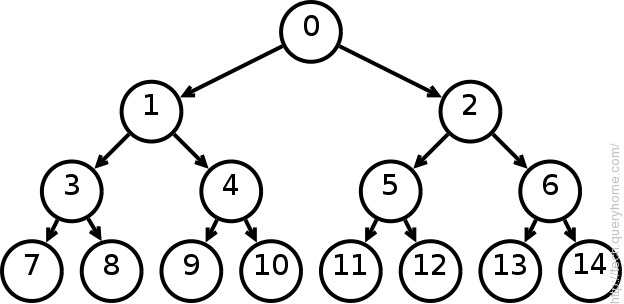
\includegraphics[scale = .75]{tree.png}
	\end{figure}
This is a geometric series, $\frac{n^{2}}{2^{i}}$, So our asymptotic upper bound of T(n) = T(n/2) + n$^{2}$ is approximately O(n$^{2}$)
\subsection{Use the master method to solve T(n) = 2T(n/4) + 1.}
Master's Theorem:\\
T(n) = aT($\frac{n}{b}$) + f(n)\\
Where, a $\geq$ 1, b $>$ 1, f(n) is asymptotically positive\\
\\
T(n) = 2T(n/4) + 1\\
a = 2, b = 4, f(n) = 1\\
n$^{log_{b}a}$ $\Rightarrow$ n$^{log_{4}2}$ $\Rightarrow$ n$^{1/2}$\\
Case 1:\\
if f(n) = O(n$^{log_{b}a - \epsilon}$) for some $\epsilon > 0$ then T(n) = $\Theta$( n$^{1/2}$).\\
Therefore, T(n) =  $\Theta$($\sqrt{n}$)

\subsection{Use the master method to solve T(n) = 2T(n/4) + $\sqrt{n}$.}
Master's Theorem:\\
T(n) = aT($\frac{n}{b}$) + f(n)\\
Where, a $\geq$ 1, b $>$ 1, f(n) is asymptotically positive\\
\\
T(n) = 2T(n/4) + $\sqrt{n}$\\
a = 2, b = 4, f(n) = $\sqrt{n}$\\
n$^{log_{b}a}$ $\Rightarrow$ n$^{log_{4}2}$ $\Rightarrow$ n$^{1/2}$\\
Case 2:\\
if f(n) is $\theta$(n$^{log_{b}a}$) then T(n) = $\theta$(n$^{log_{b}a}$lgn)\\
Therefore, T(n) = $\theta$($\sqrt{n}$lgn)\\

\subsection{Use the master method to solve T(n) = 2T(n/4) + n}
Master's Theorem:\\
T(n) = aT($\frac{n}{b}$) + f(n)\\
Where, a $\geq$ 1, b $>$ 1, f(n) is asymptotically positive\\
\\
T(n) = 2T(n/4) + n\\
a = 2, b = 4, f(n) = n\\
n$^{log_{b}a}$ $\Rightarrow$ n$^{log_{4}2}$ $\Rightarrow$ n$^{1/2}$\\
Case 3:
if f(n) is $\Omega$(n$^{log_{b}a + \epsilon}$) for some $\epsilon > 0$ and if f(n/b) $\leq$ f(n), then T(n) = $\theta(f(n))$\\
Therefore, T(n) = $\theta$(n)

\section{Suppose that the random choice of vertex always chooses the vertex with the smallest index. What are the return values of each recursive call?}
  \begin{algorithm}\caption{\textsc{SEB}}\label{alg:seb}
 \begin{algorithmic}[1]
   \State {\bf Input:} $S$, $\Sigma$
   \State {\bf Output:} $B$, the smallest ball enclosing $S$ with points of 
$\Sigma$ on the boundary.
   \State ~

   \If{$|S|=0$}
   \State Compute the smallest ball with $\Sigma$ on boundary
   \EndIf
   
   \State $i \gets \textsc{Random}(0,n-1)$
   \State $B = \textsc{SEB}(S \backslash S[i], \Sigma)$
   \If{$S[i] \in B$}\\
   ~~~~~~\Return $B$
   \Else\\
   ~~~~~~\Return $\textsc{SEB}\left((S \backslash S[i], \Sigma \cup \{ S[i] 
\}\right)$
   \EndIf
 \end{algorithmic}
\end{algorithm}
~~~
\\
1st Return: $\emptyset$\\
2nd Return: ball centered at (4,1) radius (0)\\
3rd Return: ball centered at (2.5,1) radius (1.5)\\
4th Return: ball centered at (2.5,1) radius (1.5)\\
5th Return: ball centered at (2.5,2) radius (1.8)\\
6th Return: ball centered at (2.5,2) radius (1.8)\\
7th Return: ball centered at (4.5,2.5) radius (1.6)\\
8th Return: ball centered at (3,2.5) radius (2.5)\\
9th Return: ball centered at (3,2.5) radius (2.5)\\
10th Return: ball centered at (3,2.5) radius (2.5)\\
11th Return: ball centered at (3,2.5) radius (2.5)\\


\end{document}